\subsection{Case Studies}
\label{sec:case_study}

%--------------------------------------------------------------------%

\subsubsection{Multiagent Debate}

The Multisgent Debate framework represents a pivotal shift from individualistic reasoning toward a social-deliberative paradigm for Large Language Models \citep{du2023improvingfactualityreasoninglanguage}. In its workflow, Multiagent Debate instantiates $K$ copies of an LLM agents that independently propose answers, then enter multiple debate rounds where each agent receives the concatenated responses of the other agents and is instructed to update its own answer; the update procedure repeats until a fixed round budget is exhausted. 

\paragraph{Graph Formalization.}

We formalize the Multiagent Debate workflow as a graph $G_\text{MD}=(\mathcal{N},\mathcal{E}, \mathrm{Op})$. For a debate involving $K$ agents over $T$ rounds, the node set $\mathcal{N}$ comprises computation nodes $N_{i,t} \in \mathcal{N}_{\text{comp}}$ representing agent $i \in \{1, \dots, K\}$ at round $t \in \{1, \dots, T\}$.  The coordination logic is governed by a sequence of ensemble operators $\text{Op}_{\text{ensemble}, t} \in \text{Op}$, which aggregate agent responses and determine the final voting state. The edges set $\mathcal{E}$ is partitioned into 2 classes $\mathcal{E} = E_\text{fan-in} \cup E_\text{fan-out}$. The aggregation edges $E_\text{fan-in} := \{\langle N_{i,t}, \mathrm{Op}_{\text{ensemble},t} \rangle | i \in \{1,\dots,K\}, t \in \{1,\dots,T\}\}$ represent the GPU-to-CPU data flow where independent agent reasonings converge at the synchronization barrier. And similarly the distribution edges $E_{fanout} := \{\langle \mathrm{Op}_{\text{ensemble}, t-1}, N_{i,t} \rangle\}$ represent the CPU-to-GPU broadcast of the current debate history to all $K$ parallel agents. 

As illustrated in Figure~\ref{MAD}, this formalization results in a "diamond-chain" topology, where each round $t$ initiates with a context distribution and concludes with a synchronized aggregation. This structural view makes Multiagent Debate an archetypal instance of alternating Pattern~I and Pattern~II motifs, enabling direct application of the optimizations in Section~\ref{sec:pattern-driven_system_optimizations}.

\begin{figure}
    \centering
    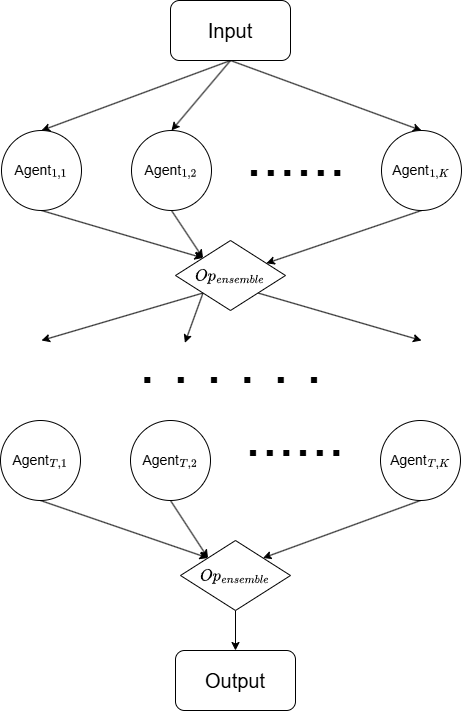
\includegraphics[width=0.5\linewidth]{./figures/MAD.drawio.png}
    \caption{Multiagent Debate}
    \label{MAD}
\end{figure}

\paragraph{Excution-level Optimizations.}

By formalizing Multiagent Debate as a typical repeating sequence of Pattern I (Fan-out) and Pattern II (Fan-in) motifs, we can map the specific structural potentials of the debate workflow to high-performance serving mechanisms.

\begin{itemize}
    \item \textbf{Context Deduplication via Radix Caching (Pattern I):} In each debate round $t$, the edge set $E_{\text{fan-out}}$ broadcasts an identical history string from $\mathrm{Op}_{\text{ens}, t-1}$ to $K$ parallel debaters. Structurally, this creates massive prefix redundancy. Rather than re-computing the KV cache for the same history $K$ times, a system like SGLang can perform a longest-prefix match against its radix tree. This reduces the total prefill complexity of the "council" from $\mathcal{O}(K \times \text{Length})$ to $\mathcal{O}(1 \times \text{Length})$, effectively neutralizing the "Prefill Shock" typically associated with multi-agent scaling.

    \item \textbf{Objective-Driven Barrier Management (Pattern II):} The aggregation edges $E_{\text{fan-in}}$ terminate at $\mathrm{Op}_{\text{ensemble}, t}$, which acts as a strict synchronization barrier; the debate cannot proceed until the slowest agent $N_{\text{slowest}, t}$ finishes its generation. This exposes a clear optimization target for the scheduler. By utilizing a DAG-aware executor like Parrot, the system can dynamically elevate the priority of the critical-path agent or utilize Sarathi-Serve's chunked-prefill to interleave its tokens with the decoding phases of faster agents. This objective-driven scheduling minimizes the idle GPU memory residency of agents who have already reached their consensus but are stuck waiting at the join barrier.
\end{itemize}

\paragraph{Graph-level Optimizations.}

While execution-level techniques optimize the existing workflow, graph-level optimizations actively mutate the topology of the Multiagent Debate to reduce unnecessary computation without degrading the quality of the consensus.

\begin{itemize}
    \item \textbf{Adaptive Subgraph Pruning via Consensus Detection (Strategy I):} The standard framework typically executes for a fixed number of rounds $T$. However, for a significant portion of queries, the agents reach a stable consensus long before the final round. By inserting a lightweight conditional operator $\text{Op}_{\text{exit}}$ after the ensemble node $\text{Op}_{\text{ens}, t}$, the system can perform real-time consensus detection. If the debaters $\{N_{1,t}, \dots, N_{K,t}\}$ converge on the same answer, all downstream nodes $\{N_{i, t+1}, \dots, N_{i, T}\}$ and their associated edges are pruned from the execution graph. This Adaptive Subgraph Pruning reclaims GPU memory and compute cycles that would otherwise be wasted on redundant "agreement" rounds.

    \item \textbf{Heterogeneous Node Downscaling (Strategy II):} The "star" topology in the framework often treats all debaters as homogeneous frontier models. In practice, the early "brainstorming" rounds can be handled by task-specialized Small Language Models that generate diverse perspectives at a fraction of the cost. For instance, we can replace the debator nodes with smaller models with different persona, reserving the primary large model only for the final rounds.

    \item \textbf{Subgraph Consolidation for Low-Complexity Queries (Strategy IV):} For queries identified as "easy" (e.g., via a difficulty estimator like DAAO), the entire multi-round debate subgraph can be collapsed into a single consolidated node $N_{\text{consolidated}}$. This node uses a highly capable model to simulate a "Multi-perspective Chain-of-Thought" in a single forward pass. Consolidation eliminates the inter-agent communication overhead of the $E_{\text{fan-in}}/E_{\text{fan-out}}$ cycles entirely and maximizes KV cache reuse, offering a high-throughput alternative for non-adversarial tasks.
\end{itemize}

Multiagent Debate is a canonical ``diamond-chain'' instance of alternating Fan-out and Fan-in motifs. This topology makes (i) prefix redundancy and (ii) barrier tail latency inevitable at execution time, while also enabling graph-level cost reductions through early exits, heterogeneous model assignment, and conditional consolidation. In this sense, the debate framework serves as a compact case study demonstrating how structural visibility in $G=(\mathcal{N},\mathcal{E},\mathrm{Op})$ directly translates into actionable system and graph optimizations.

%--------------------------------------------------------------------%

\subsubsection{MetaGPT}
The MetaGPT framework represents a software-engineering-inspired coordination paradigm \citep{hong2023metagpt}. Unlike the homogeneous reasoning in Multiagent Debate, MetaGPT introduces five specialized agent roles (Product Manager, Architect, Project Manager, Engineer, and QA Engineer). These roles are coordinated through Standard Operating Procedures (SOPs), forming a structured pipeline where agents asynchronously refine shared artifacts via a Publish–Subscribe mechanism over a Global Message Pool. 

\paragraph{Graph Formalization.}

We formalize the MetaGPT workflow as a graph $G_{\text{MetaGPT}} = (\mathcal{N}, \mathcal{E}, \mathrm{Op})$.
The node set $\mathcal{N}$ is heterogeneous, comprising both specialized computation nodes and functional tool nodes. Specifically, the computation node set is defined as $\mathcal{N}{\text{compute}} = \{N_{\text{PM}}, N_{\text{Arch}}, N_{\text{ProjM}}, N_{\text{Eng}}, N_{\text{QA}}\}$, where each node represents a role-specialized agent in the software development lifecycle. Additionally, the tool node set is defined as $\mathcal{N}{\text{tool}} = \{N_{\text{search}}, N_{\text{debug}}, N_{\text{diagram}}\}$, which provides deterministic external functionalities such as web information search, execution debugging, and system visualization. The full node set is therefore given by $\mathcal{N} = \mathcal{N}{\text{compute}} \cup \mathcal{N}{\text{tool}}$.
% The edge set $\mathcal{E}$ is partitioned into three distinct classes that govern both inter-role coordination and intra-role reasoning dynamics, namely $\mathcal{E} = E_{\text{seq}} \cup E_{\text{int}} \cup E_{\text{ref}}$.
The edge set $\mathcal{E}$ is partitioned into two distinct classes, namely $\mathcal{E} = E_{\text{int}} \cup E_{\text{ref}}$.
% \begin{itemize}
%     \item \textbf{Sequential Pipeline Edges ($E_{\text{seq}}$):}  These edges represent the macro-level SOP flow between specialized roles. An edge $\langle N_i, N_j \rangle \in E_{\text{seq}}$ exists when node $N_j$ subscribes to structured artifacts published by node $N_i$ through the shared message pool. 
%     \item \textbf{Compute-Tool Interleaving Edges ($E_{\text{int}}$):} These edges enable interaction between computation nodes and tool nodes. For example, $\langle N_{\text{PM}}, N_{\text{search}} \rangle \in E_{\text{int}}$ allows the Product Manager to retrieve web information.
%     \item \textbf{Iterative Reflection Edges ($E_{\text{ref}}$):} Within the Engineer node $N_{\text{Eng}}$, the agent generates a code artifact that is evaluated by an execution operator $\mathrm{Op}_{\text{eval}} \in \mathrm{Op}$. If the evaluation feedback indicates errors or constraint violations, a reflection edge $\langle \mathrm{Op}_{\text{eval}}, N_{\text{Eng}} \rangle \in E_{\text{ref}}$ routes the feedback back to the agent, enabling iterative refinement.
% \end{itemize}

\begin{itemize} 
    \item \textbf{Compute-Tool Interleaving Edges ($E_{\text{int}}$):} These edges enable interaction between computation nodes and tool nodes. For example, $\langle N_{\text{PM}}, N_{\text{search}} \rangle \in E_{\text{int}}$ allows the Product Manager to retrieve web information.
    \item \textbf{Iterative Reflection Edges ($E_{\text{ref}}$):} Within the Engineer node $N_{\text{Eng}}$, the agent generates a code artifact that is evaluated by an execution operator $\mathrm{Op}_{\text{eval}} \in \mathrm{Op}$. If the evaluation feedback indicates errors or constraint violations, a reflection edge $\langle \mathrm{Op}_{\text{eval}}, N_{\text{Eng}} \rangle \in E_{\text{ref}}$ routes the feedback back to the agent, enabling iterative refinement.
\end{itemize}

\begin{figure}
    \centering
    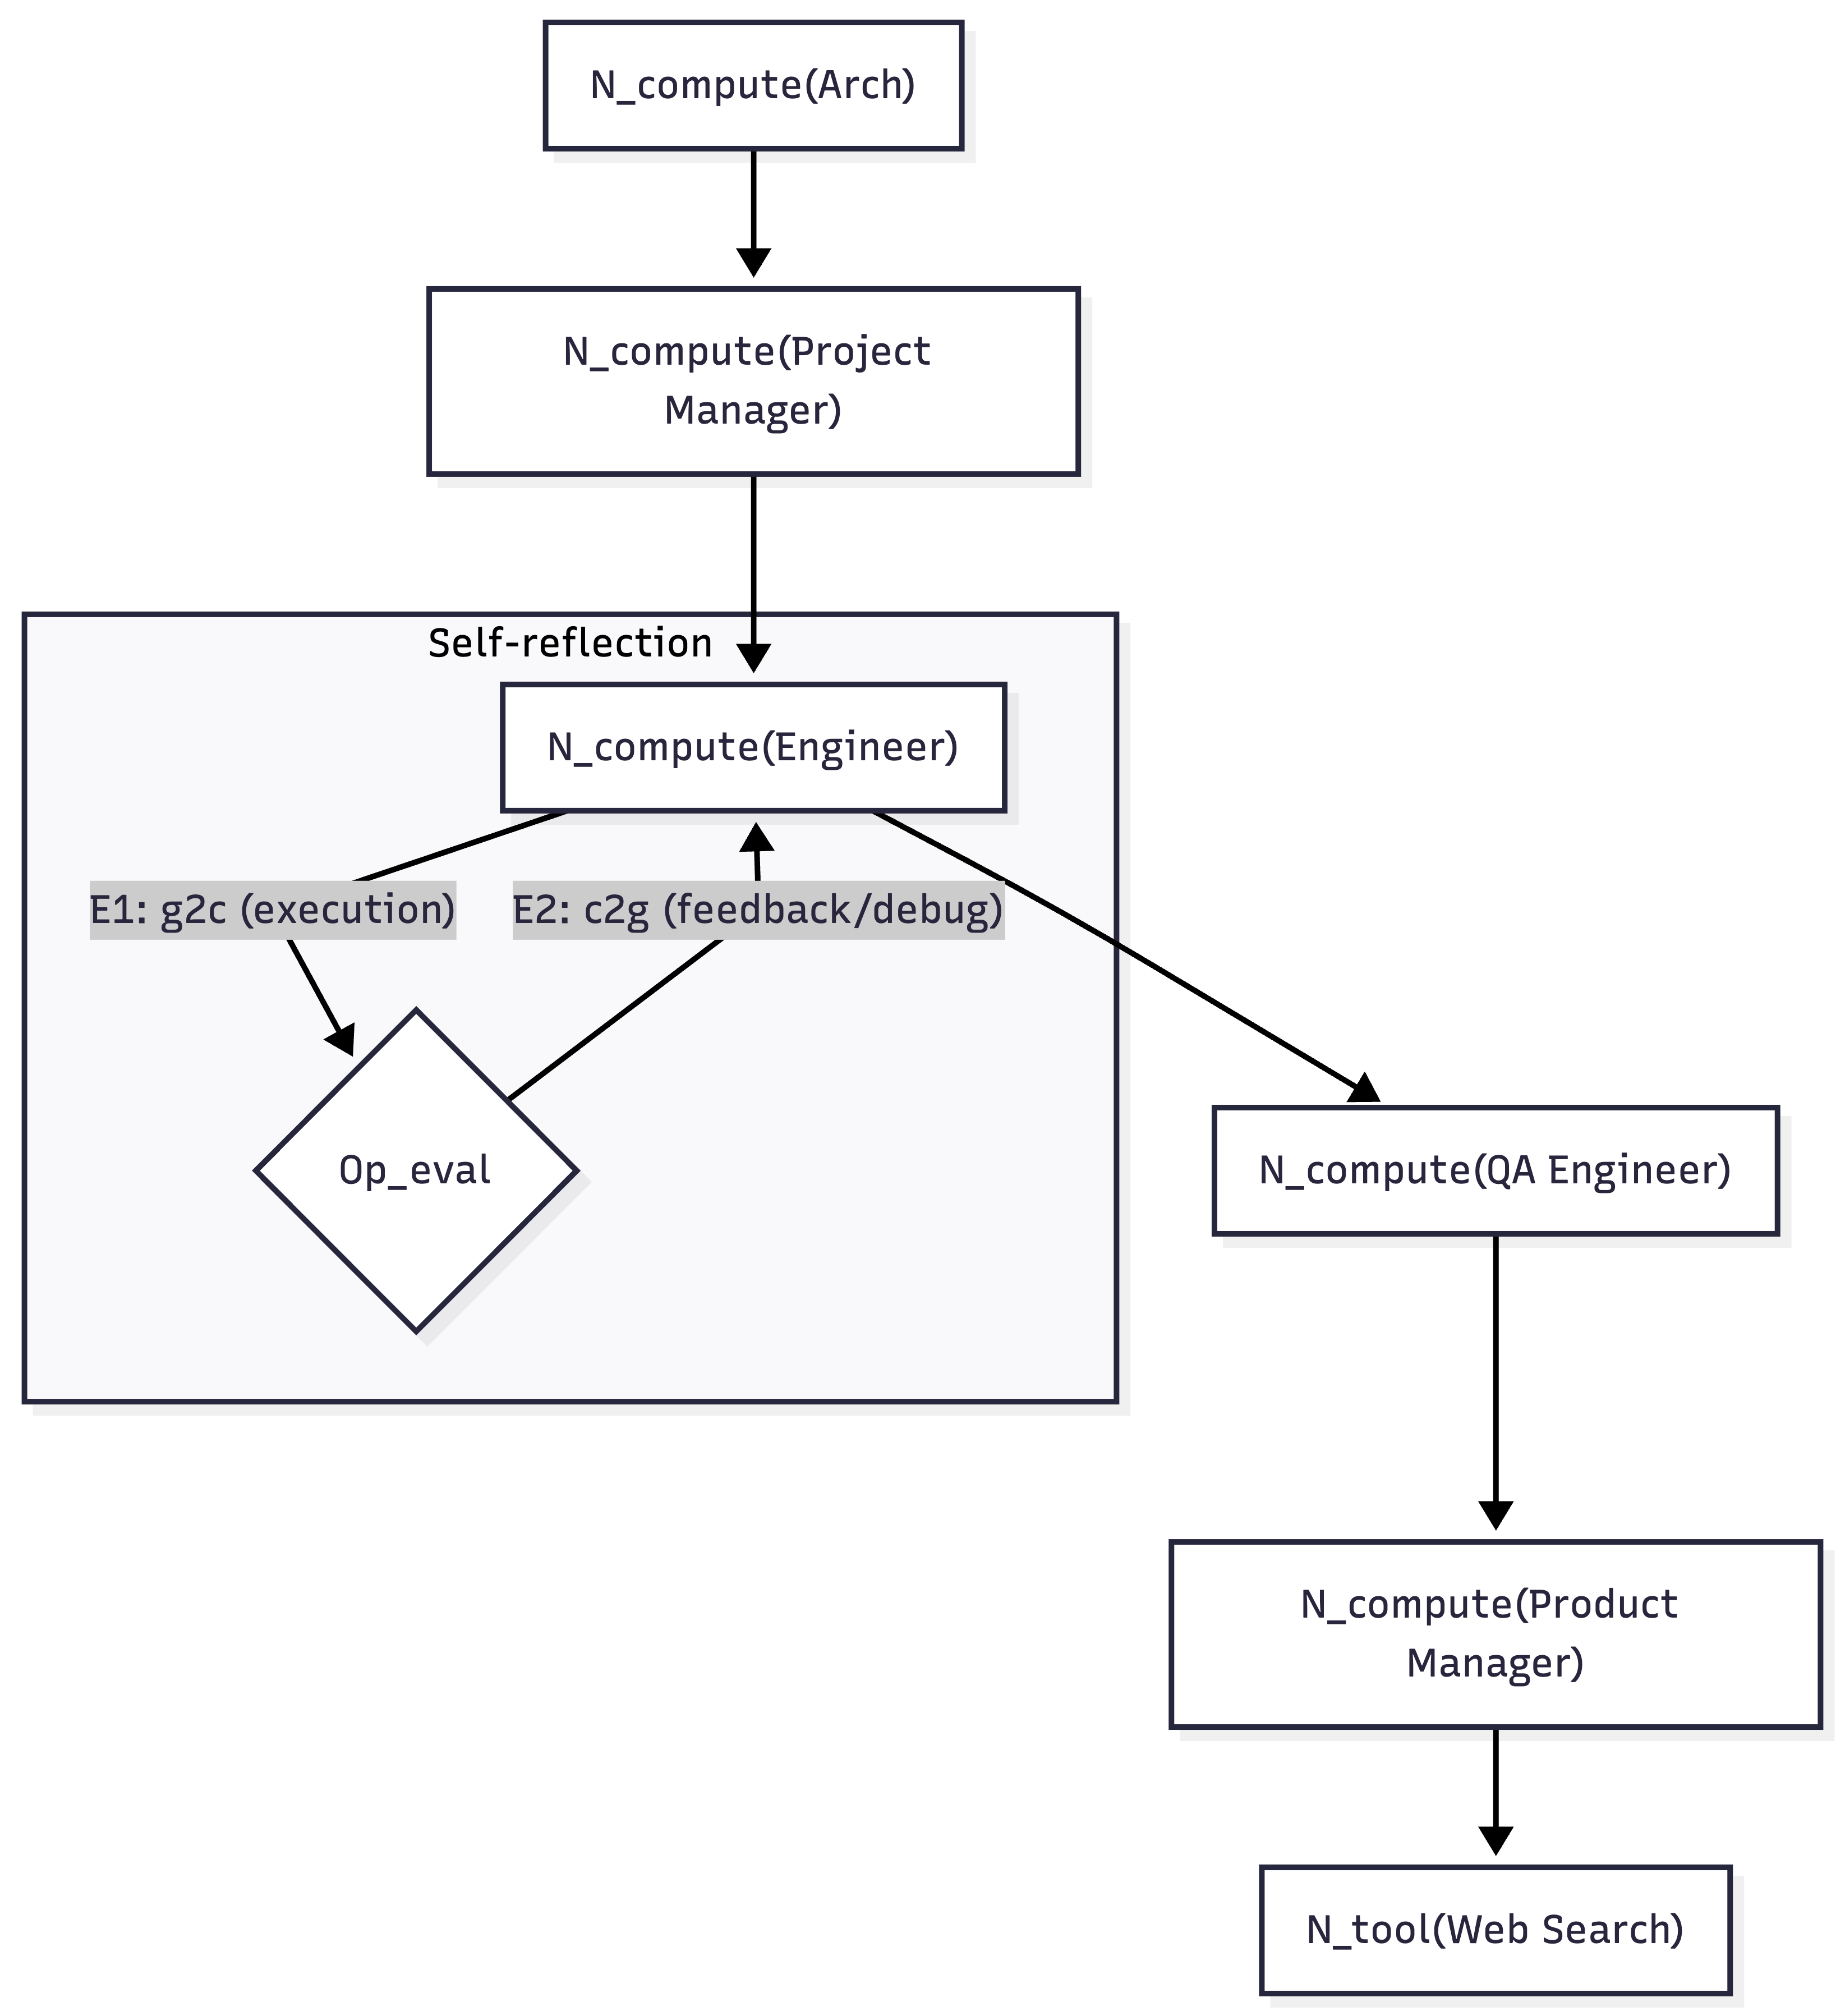
\includegraphics[width=0.5\linewidth]{./figures/metagpt.png}
    \caption{MetaGPT}
    \label{MGPT}
\end{figure}

% As illustrated in Figure~\ref{MGPT}, this formalization characterizes MetaGPT as an artifact-driven pipeline, where the execution flow is governed by structured dependencies between heterogeneous nodes. This structural view identifies MetaGPT as a canonical instance of Pattern III (Sequential Pipeline) at the macro level. At the intra-node level, the architecture incorporates Pattern V (Heterogeneous Interleaving). Specifically, the Engineer node $N_{\text{Eng}}$ further integrates Pattern IV (Iterative Reflection). These structures enable the direct application of the optimizations in Section~\ref{sec:pattern-driven_system_optimizations}.
As illustrated in Figure~\ref{MGPT}, this formalization characterizes MetaGPT as an artifact-driven pipeline, where the execution flow is governed by structured dependencies between heterogeneous nodes. This structural view identifies MetaGPT as a role-specialized multi-agent pipeline at the macro level.
At the intra-node level, the architecture incorporates Pattern V (Heterogeneous Interleaving). Specifically, the Engineer node $N_{\text{Eng}}$ further integrates Pattern III (Iterative Reflection). These structures enable the direct application of the optimizations in Section~\ref{sec:pattern-driven_system_optimizations}.

\paragraph{Excution-level Optimizations.}
By mapping the MetaGPT workflow to a combination of Pattern V (Interleaving), and III (Reflection), we can exploit its structural determinism and role-specialization to optimize resource utilization and latency.

% \begin{itemize}
%     \item \textbf{Proactive KV-Prefetching via SOP Determinism (Pattern III):} The MetaGPT workflow is governed by a strict SOP where the transition between specialized roles is topologically deterministic via $E_{\text{seq}}$. Unlike stochastic branching, the transition probability (e.g., from $N_{\text{Arch}}$ to $N_{\text{ProjM}}$) is near $1.0$. This allows the system to utilize KVFlow-style optimizations: while the $N_{\text{Arch}}$ node is generating the System Design, the system can proactively prefetch the massive, role-specific system prompts and historical context for the upcoming $N_{\text{ProjM}}$ node from host memory to GPU. By overlapping KV-cache loading with the decoding phase of the preceding agent, the system hides the "cold-start" latency of heterogeneous role transitions.
%    \item \textbf{Proactive Memory Yielding during Tool Latency (Pattern VI):} The interleaving edges $E_{\text{int}}$ between $\mathcal{N}_{\text{compute}}$ and $\mathcal{N}_{\text{tool}}$ introduce significant GPU idle time, particularly during long-running tasks like $N_{\text{search}}$ or complex $N_{\text{debug}}$ sessions. Since $N_{\text{tool}}$ nodes do not require Tensor Core compute, they represent a perfect "yield trigger." A DAG-aware executor like Parrot can detect the traversal of an $E_{\text{int}}$ edge and immediately trigger a proactive swap-out of the calling agent's KV cache to CPU memory. This transforms the unpredictable tool execution latency from a "memory-hogging" wait state into a resource-reclaiming opportunity, allowing concurrent requests to utilize the freed GPU memory.
%    \item \textbf{Context Pinning for Debugging Cycles (Pattern IV):} Within the Engineer node $N_{\text{Eng}}$, the iterative reflection edges $E_{\text{ref}}$ create a high-locality loop during code refinement. Although the error feedback changes, the underlying codebase and task instructions remain invariant. By utilizing programmable cache controllers like Pie, the system can "pin" the foundational KV-pages of the current code artifact. During the $\langle \mathrm{Op}_{\text{eval}}, N_{\text{Eng}} \rangle$ feedback loop, the system avoids re-computing the prefill for the entire file, reducing the iterative refinement latency to the cost of processing only the new feedback tokens.
%    \item \textbf{Role-based Disaggregated Serving (Pattern V variant):} MetaGPT displays structural asymmetry between "manager" nodes (which process large context summaries like PRDs or System Designs) and "worker" nodes (which generate specific code snippets). Following the principles of Splitwise, $N_{\text{Arch}}$ and $N_{\text{ProjM}}$ nodes, which are prefill-heavy due to large document ingestion, can be scheduled on compute-optimized instances (e.g., H100), while $N_{\text{Eng}}$ nodes, which are decode-heavy during code generation, can be placed on memory-bandwidth-optimized instances.
% \end{itemize}
\begin{itemize}
   \item \textbf{Proactive Memory Yielding during Tool Latency (Pattern V):} The interleaving edges $E_{\text{int}}$ between $\mathcal{N}_{\text{compute}}$ and $\mathcal{N}_{\text{tool}}$ introduce GPU idle time, particularly during long-running tasks like $N_{\text{search}}$ or complex $N_{\text{debug}}$ sessions. Since $N_{\text{tool}}$ nodes do not require Tensor Core compute, they represent a perfect "yield trigger." A DAG-aware executor like Parrot can detect the traversal of an $E_{\text{int}}$ edge and immediately trigger a proactive swap-out of the calling agent's KV cache to CPU memory. This transforms the unpredictable tool execution latency from a "memory-hogging" wait state into a resource-reclaiming opportunity, allowing concurrent requests to utilize the freed GPU memory.
   \item \textbf{Context Pinning for Debugging Cycles (Pattern III):} Within the Engineer node $N_{\text{Eng}}$, the iterative reflection edges $E_{\text{ref}}$ create a high-locality loop during code refinement. Although the error feedback changes, the underlying codebase and task instructions remain invariant. By utilizing programmable cache controllers like Pie, the system can "pin" the foundational KV-pages of the current code result. During the feedback loop, the system avoids re-computing the prefill for the entire file, reducing the iterative refinement latency to the cost of processing only the new feedback tokens.
\end{itemize}

\paragraph{Graph-level Optimizations.}
While execution-level techniques optimize the performance of the existing pipeline, graph-level optimizations actively mutate the MetaGPT topology to eliminate structural redundancies inherent in its software-engineering-inspired development process. 
\begin{itemize}
    \item \textbf{Adaptive Pipeline Pruning via Task Complexity Estimation (Strategy I):}The full MetaGPT SOP is often over-engineered for simple requests (e.g., "Write a Python script to sort a CSV"). By inserting a conditional $\text{Op}_{\text{exit}}$ node after the initial requirement analysis in $N_{\text{Arch}}$, the system can assess the task's structural complexity. This "fast-track" execution routes the requirement directly to $N_{\text{Eng}}$, eliminating the token costs and latency of intermediate high-level design stages that add no value to trivial implementations.
    \item \textbf{Heterogeneous Role-Model Alignment (Strategy II):} MetaGPT's heterogeneity is currently defined by agent personas, but it often utilizes a homogeneous frontier model (GPT-4o) for all roles. We can optimize this by performing \textbf{node-level downscaling}: assigning different computational backends to $N_i$ based on the functional entropy of the role. For instance, while $N_{\text{Arch}}$ requires the global reasoning and creative capacity of a large frontier model to handle system-wide trade-offs, the $N_{\text{QA}}$ and $N_{\text{Eng}}$ nodes can be replaced with task-specialized SLMs (e.g., a 7B-parameter DeepSeek-Coder). This strategy exploits the observation that role-specific fine-tuning on smaller models can match or exceed generalist performance in structured tasks.
    \item \textbf{Sparse Expert Dispatch for Multi-Stack Projects (Strategy III):} Large-scale software projects often involve multiple technology stacks (e.g., React frontend and Go backend). Rather than using a single $N_{\text{Eng}}$ node, we can decompose the Engineering phase into a sparse expert subgraph. A $N_{\text{router}}$ node analyzes the $N_{\text{ProjM}}$'s task list and selectively activates expert nodes $\{\mathcal{E}_{\text{frontend}}, \mathcal{E}_{\text{backend}}, \mathcal{E}_{\text{devops}}\}$. This prevents "context pollution" within a single engineer agent and allows for expert parallelism, where different stack-specialized agents can execute concurrently on hardware instances optimized for their specific language models.
\end{itemize}

\section{Extended Discussion of Graph-Level Optimizations}
\label{app:graph_level_optimizations_extended}

This appendix provides additional technical detail and literature context for the graph-level optimization strategies introduced in Section~\ref{sec:graph_level_optimizations}.

\subsection{Adaptive Subgraph Pruning}

Adaptive Subgraph Pruning is motivated by a simple empirical fact: not all queries require the full depth of a multi-agent workflow. In realistic deployments, query difficulty is highly skewed, and many instances can be handled correctly by early-stage agents without engaging the full pipeline of drafting, critique, refinement, and verification. Running every query through the complete graph therefore creates systematic overcomputation.

First, pruning downstream nodes directly reduces the number of LLM invocations. If a pipeline of depth $k$ exits after stage $j$, the system avoids $(k-j)$ additional forward passes. Second, the savings are often superlinear in tokens because later agents usually consume the accumulated outputs of earlier agents. Skipping later stages avoids not only their generation cost but also the growth of prefill cost caused by increasingly long prompts. Third, pruning improves memory efficiency: KV caches for skipped nodes are never allocated, and completed caches can often be freed earlier because no downstream consumer remains.

This pattern is supported by several lines of prior work. At the model level, LayerSkip~\citep{elhoushi2024layerskip} and AdaInfer~\citep{fan2024adainfer} show that inputs of different difficulty can profitably use different effective depths. At the routing level, FrugalGPT~\citep{chen2023frugalgpt}, RouteLLM~\citep{ong2024routellm}, AutoMix~\citep{aggarwal2024automix}, and Hybrid LLM~\citep{ding2024hybridllm} similarly apply adaptive escalation across models. At the workflow level, DAAO~\citep{daao2025} constructs simpler workflows for easy queries and richer ones for hard queries, while MaAS~\citep{zhang2025maas} samples query-dependent subnetworks from an agentic supernet. STIG~\citep{stig2025} shows that in structured settings the strongest form of pruning may collapse the entire workflow to a single call. Related evidence from adaptive debugging systems~\citep{adaptive_debug2025} also supports the claim that easy instances benefit from minimal agentic depth whereas difficult ones benefit from additional collaboration.

\subsection{Heterogeneous Node Downscaling}

Heterogeneous Node Downscaling addresses a recurring architectural mismatch in multi-agent systems: different nodes often perform narrow specialized functions, yet many frameworks instantiate every node with the same large frontier model. This homogeneous design over-provisions compute for roles such as summarization, formatting, verification, parsing, or constrained tool invocation.

The systems benefits are straightforward. Replacing a large model with a smaller one at even a single node reduces FLOPs per invocation substantially. Smaller models also reduce memory footprint and KV-cache growth, improving concurrency and lowering infrastructure cost. Because small language models are easier to fine-tune or adapt with lightweight methods such as LoRA, the workflow graph also creates a natural path toward progressive specialization: once the role of a node is observed repeatedly, the system can replace a generalist LLM with a right-sized specialist.

The literature supports this view from multiple angles. Distilling Step-by-Step~\citep{hsieh2023distilling} and MiniLLM~\citep{gu2023minillm} establish the feasibility of transferring task-relevant capabilities from large to small models. Belcak et al.~\citep{belcak2025slm} argue that many agentic tasks are better matched to SLMs than to frontier LLMs and propose an explicit LLM-to-SLM conversion process based on usage clustering and iterative specialization. X-MAS~\citep{ye2025xmas} finds that no single model dominates across all functions and domains, providing direct evidence for heterogeneous assignment. DAAO~\citep{daao2025} further operationalizes node-level routing to different models. BudgetMLAgent~\citep{budgetmlagent2024} shows that replacing most worker calls with cheaper models can dramatically reduce cost while maintaining or improving success rate. From a serving perspective, this strategy aligns naturally with disaggregated systems such as Splitwise~\citep{patel2024splitwise} and DistServe~\citep{zhong2024distserve}, which already separate phases or resource profiles across hardware tiers.

\subsection{Sparse Expert Decomposition}

Sparse Expert Decomposition generalizes the mixture-of-experts principle from model internals to workflow structure. Instead of using one dense agent for all query types, the system replaces that node with a router and a collection of smaller experts. Only a small subset of experts is activated for each query, after which their outputs are aggregated and passed forward.

This yields several systems advantages. First, it creates sparse activation at the agent level, so the active compute per request becomes a function of the selected experts rather than the full capacity of a generalist node. Second, it encourages more focused specialization, since each expert can target a narrow subtask such as numerical reasoning, SQL generation, citation formatting, or data extraction. Third, because experts are smaller, they can be distributed flexibly across devices or replicated asymmetrically according to demand, connecting the workflow abstraction to hardware-aware scheduling.

This idea is grounded in successful model-level MoE systems such as Switch Transformer~\citep{fedus2022switch}, Mixtral~\citep{jiang2024mixtral}, and DeepSeek-V3~\citep{deepseekai2025deepseekv3}, all of which show that sparse activation can provide very large total capacity at much lower active compute. At the workflow level, DAAO~\citep{daao2025} can be interpreted as a router selecting among heterogeneous operator-model pairs, while MaAS~\citep{zhang2025maas} provides an especially direct analogue via query-dependent sampling of a subnetwork from an agentic supernet. From a systems standpoint, this makes the router simultaneously a capability selector and a placement decision-maker, closely resembling expert parallelism strategies such as MegaBlocks~\citep{gale2023megablocks}.

\subsection{Subgraph Consolidation}

Subgraph Consolidation is the inverse of pruning and the dual of expert decomposition: instead of expanding or selectively skipping structure, it collapses an existing multi-agent region into a single node executed by a stronger model. This is motivated by the growing observation that many multi-agent workflows, especially homogeneous ones, incur coordination and communication overhead without clear gains in quality.

The systems benefits are threefold. First, consolidation eliminates internal communication edges, removing serialization, deserialization, and network or process hand-off overheads. Second, it avoids context fragmentation, since the full task is processed in one coherent context rather than being split across multiple agent windows. Third, it mitigates error cascades, because intermediate outputs no longer serve as brittle interfaces between stages.

Several recent works support this pattern. OneFlow~\citep{xu2026oneflow} shows that homogeneous multi-agent workflows can often be simulated by a single LLM through multi-turn internalized execution, with the added benefit of KV-cache reuse. AgentArk~\citep{luo2026agentark} demonstrates that debate-style multi-agent behavior can be distilled into a single model’s parameters, shifting orchestration cost from inference time to training time. Chain-of-Agents~\citep{li2025chainofagents} similarly distills multi-agent trajectories into agent foundation models that can outperform the original systems. STIG~\citep{stig2025} provides a domain-specific example in which a multi-stage academic writing workflow is replaced by a single model equipped with stage tokens. From a serving perspective, consolidated execution often maps better to systems such as Splitwise~\citep{patel2024splitwise} and DistServe~\citep{zhong2024distserve}, which benefit from sustained long-context execution rather than many short fragmented calls.

That said, consolidation is not universally appropriate. It works best when the subgraph is relatively homogeneous, when the entire relevant context fits within the large model’s window, and when one model can adequately subsume the constituent functions. When these conditions do not hold, the decomposed architecture may remain preferable. This motivates conditional consolidation, where the runtime profiles subgraphs and consolidates only those whose expected quality loss remains below a chosen threshold.